%%%%%%%%%%%%%%%%%%%%%%%%%%%%%%%%%%%%%%%%%%%%%%%%%%%%%%%%%%%%%%%%%%%%%%%%%%%%%%%%
% Template IEEE - MIEI @ Universidade de Coimbra
% Baseado no template oficial do IEEE
%%%%%%%%%%%%%%%%%%%%%%%%%%%%%%%%%%%%%%%%%%%%%%%%%%%%%%%%%%%%%%%%%%%%%%%%%%%%%%%%

% Define a classe do documento. 'conference' usa o formato standard de 2 colunas.
\documentclass[conference]{IEEEtran}

% --- PACOTES ESSENCIAIS ---

% Para lidar com acentuação e caracteres especiais
\usepackage[utf8]{inputenc}
\usepackage[T1]{fontenc}

% Para matemática
\usepackage{amsmath, amsfonts, amssymb}

% Para incluir gráficos (imagens)
\usepackage{graphicx}
% Adicionado para \rotatebox
\usepackage{rotating} 

% Para gestão de citações (estilo IEEE)
% NOTA: O 'IEEEtran' já faz muito disto, mas 'cite' ajuda a formatar [1]-[3]
\usepackage{cite}

% Para URLs
\usepackage{url}

% Para tabelas
\usepackage{booktabs} % For professional-looking tables
\usepackage{pgfplots} % Adicionado para gráficos (box plot)
\usepgfplotslibrary{statistics} % Adicionado para corrigir o erro do boxplot
\pgfplotsset{compat=1.18} % Define a versão do pgfplots

% Para texto "dummy" (placeholder) - REMOVER QUANDO ESCREVERES
\usepackage{lipsum}

% Para equilibrar as colunas na última página (importante)
\usepackage{balance}

% Para links clicáveis no PDF (recomendo 'hidelinks' para não ter caixas coloridas)
\usepackage[hidelinks]{hyperref}


%%%%%%%%%%%%%%%%%%%%%%%%%%%%%%%%%%%%%%%%%%%%%%%%%%%%%%%%%%%%%%%%%%%%%%%%%%%%%%%%
% --- CRIAÇÃO DE UM FICHEIRO .BIB (PARA COMPILAÇÃO) ---
%%%%%%%%%%%%%%%%%%%%%%%%%%%%%%%%%%%%%%%%%%%%%%%%%%%%%%%%%%%%%%%%%%%%%%%%%%%%%%%%
% Para que o documento compile, crio um ficheiro .bib de exemplo 
% com as referências que parecem ser necessárias.
\usepackage{filecontents}
\begin{filecontents*}{myreferences.bib}
@book{GoF1995,
    author    = {Gamma, Erich and Helm, Richard and Johnson, Ralph and Vlissides, John},
    title     = {Design Patterns: Elements of Reusable Object-Oriented Software},
    year      = {1995},
    publisher = {Addison-Wesley Professional},
    address   = {Reading, MA, USA},
}
@misc{DPF_Tool,
    author       = {Butt, Jonas},
    title        = {DesignPatternFinder: A tool for detecting GoF design patterns in code},
    year         = {2010},
    howpublished = {\url{https://www.softpedia.com/get/Programming/Other-Programming-Files/Design-Pattern-Finder.shtml}},
    note         = {Accessed: 2025-11-12}
}
@misc{girirajvyas2024,
    author       = {Vyas, Giriraj},
    title        = {GoF Design Patterns: Implementation of Gang of Four design patterns in Java},
    year         = {2024},
    howpublished = {\url{https://github.com/girirajvyas/gof-design-patterns}},
    note         = {Accessed: 2025-11-12}
}
@misc{ramesh2024,
    author       = {Fadatare, Ramesh},
    title        = {GoF Java Design Patterns: Complete implementation of Gang of Four design patterns in Java},
    year         = {2024},
    howpublished = {\url{https://github.com/RameshMF/gof-java-design-patterns}},
    note         = {Accessed: 2025-11-12}
}
@misc{huggingface2024,
    author       = {{Hugging Face}},
    title        = {Hugging Face: The AI community building the future},
    year         = {2024},
    howpublished = {\url{https://huggingface.co/}},
    note         = {Accessed: 2025-11-12}
}
% --- Correctness ---
@inproceedings{TongZhang2024,
    author       = {Tong, Zhaowei and Zhang, Jingbo},
    title        = {CodeJudge: Evaluating Code Generation with Large Language Models},
    booktitle    = {Proceedings of the 2024 Conference on Empirical Methods in Natural Language Processing (EMNLP)},
    year         = {2024},
    publisher    = {Association for Computational Linguistics},
    howpublished = {\url{https://aclanthology.org/2024.emnlp-main.1118.pdf}},
    note         = {Accessed: 2025-11-12}
}
@article{L2CEval2024,
    author       = {Chen, Shuxin and Chen, Simeng and others},
    title        = {L2CEval: Evaluating Language-to-Code Generation Capabilities of Large Language Models},
    journal      = {Transactions of the Association for Computational Linguistics},
    year         = {2024},
    publisher    = {MIT Press},
    howpublished = {\url{https://direct.mit.edu/tacl/article/doi/10.1162/tacl_a_00705/124835/L2CEval-Evaluating-Language-to-Code-Generation}},
    note         = {Accessed: 2025-11-12}
}
@misc{SharmaDavid2025,
    author       = {Sharma, Arindam and David, Cristina},
    title        = {Assessing Correctness in LLM-Based Code Generation via Uncertainty Estimation},
    year         = {2025},
    howpublished = {\url{https://arxiv.org/abs/2502.11620}},
    note         = {arXiv preprint arXiv:2502.11620, Accessed: 2025-11-12}
}
% --- Efficiency ---
@misc{Qiu2024,
    author       = {Qiu, Yifan and Zhang, Rui and others},
    title        = {How Efficient is LLM-Generated Code? A Rigorous and High-Standard Benchmark},
    year         = {2024},
    howpublished = {\url{https://arxiv.org/abs/2406.06647}},
    note         = {arXiv preprint arXiv:2406.06647, Accessed: 2025-11-12}
}
@misc{Huang2024,
    author       = {Huang, Xiang and Li, Bowen and others},
    title        = {EffiBench: Benchmarking the Efficiency of Automatically Generated Code},
    year         = {2024},
    howpublished = {\url{https://arxiv.org/abs/2402.02037}},
    note         = {arXiv preprint arXiv:2402.02037, Accessed: 2025-11-12}
}
% --- Maintainability ---
@misc{Yang2024,
    author       = {Yang, Tianyu and Xu, Jing and others},
    title        = {Evaluating the Generalization Capabilities of Large Language Models on Code Reasoning and Maintainability},
    year         = {2024},
    howpublished = {\url{https://www.emergentmind.com/papers/2401.12714}},
    note         = {Accessed: 2025-11-12}
}
% --- Pattern Detection Ability ---
@article{Pandey2025,
    author       = {Pandey, Rajesh and Chand, Shreya and Groenewegen, Danny and Vasilescu, Bogdan},
    title        = {Design Pattern Recognition: A Study of Large Language Models},
    journal      = {Empirical Software Engineering},
    year         = {2025},
    publisher    = {Springer},
    howpublished = {\url{https://link.springer.com/article/10.1007/s10664-025-10625-1}},
    note         = {Accessed: 2025-11-12}
}
\end{filecontents*}
%%%%%%%%%%%%%%%%%%%%%%%%%%%%%%%%%%%%%%%%%%%%%%%%%%%%%%%%%%%%%%%%%%%%%%%%%%%%%%%%


%%%%%%%%%%%%%%%%%%%%%%%%%%%%%%%%%%%%%%%%%%%%%%%%%%%%%%%%%%%%%%%%%%%%%%%%%%%%%%%%
% --- INFORMAÇÃO DO ARTIGO ---
%%%%%%%%%%%%%%%%%%%%%%%%%%%%%%%%%%%%%%%%%%%%%%%%%%%%%%%%%%%%%%%%%%%%%%%%%%%%%%%%

% Título do Artigo
\title{Design Patterns and LLMs}

% Informação dos Autores
\author{
    \IEEEauthorblockN{Francisco Pereira, Gonçalo Borges, Tiago Mendes}
    \IEEEauthorblockA{\textit{Masters in Computer Science - Software Engineering} \\
    \textit{Faculdade de Ciências e Tecnologias da Universidade de Coimbra}\\
    Coimbra, Portugal \\
    Email: \{uc2022217071, uc2022215524, uc2022216857\}@student.uc.pt}
}

% Comandos especiais do IEEE (ex: para copyright notice, se necessário)
% \IEEEoverridecommandlockouts
% \IEEEpubid{\makebox[\columnwidth]{978-X-XXXX-XXXX-X/XX/\$XX.00 \copyright 20XX IEEE \hfill} \hspace{\columnsep}\makebox[\columnwidth]{ }}


%%%%%%%%%%%%%%%%%%%%%%%%%%%%%%%%%%%%%%%%%%%%%%%%%%%%%%%%%%%%%%%%%%%%%%%%%%%%%%%%
% --- INÍCIO DO DOCUMENTO ---
%%%%%%%%%%%%%%%%%%%%%%%%%%%%%%%%%%%%%%%%%%%%%%%%%%%%%%%%%%%%%%%%%%%%%%%%%%%%%%%%
\begin{document}

% Cria o título, autores e afiliação
\maketitle

% --- ABSTRACT ---
\begin{abstract}
The architectural quality of code generated by Large Language Models (LLMs) is a critical but largely unexplored dimension. While LLMs produce functional code, their autonomous adoption of established "Gang of Four" (GoF) software design patterns is unknown. This paper presents the first empirical study to quantify the spontaneous emergence of the 23 GoF patterns in LLM-generated Java code. We analyzed a 600-file corpus generated by six different LLMs from 100 neutral prompts, using a validated analysis tool.

Our findings show a strong bias towards simplicity. Only 18.2\% of files contained any GoF pattern, and only 10 of the 23 patterns were ever detected. A heavy concentration (nearly 78\%) was found on just three patterns: Builder, State, and Command. Notably, 13 fundamental patterns, including Observer and Composite, were completely absent. We conclude that current LLMs do not make sophisticated, autonomous design decisions, instead reflecting common statistical patterns from their training data, which raises concerns about the maintainability of the code they produce for complex systems.

\end{abstract}

% Espaço entre parágrafos
\setlength{\parskip}{1em}

% --- KEYWORDS ---
% Opcional, mas recomendado
\begin{IEEEkeywords}
Large Language Models (LLMs)
Design Patterns
Gang of Four (GoF)
Code Generation
Code Analysis
Software Engineering
Empirical Study
Java
\end{IEEEkeywords}

%%%%%%%%%%%%%%%%%%%%%%%%%%%%%%%%%%%%%%%%%%%%%%%%%%%%%%%%%%%%%%%%%%%%%%%%%%%%%%%%
% --- SECÇÕES DO ARTIGO ---
%%%%%%%%%%%%%%%%%%%%%%%%%%%%%%%%%%%%%%%%%%%%%%%%%%%%%%%%%%%%%%%%%%%%%%%%%%%%%%%%

% --- I. INTRODUÇÃO ---
\section{Introduction}
% A introdução define o contexto do trabalho.
% 1. Qual é o problema?
% 2. Porque é que é importante?
% 3. Qual é o estado da arte (muito brevemente)?
% 4. Qual é a tua contribuição/proposta?
% 5. Como está o resto do artigo estruturado?

Large Language Models (LLMs) have recently become powerful tools for automated code generation, assisting developers in solving programming tasks in a wide range of domains. Modern models are capable of producing syntactically correct and functionally accurate programs from natural-language prompts. While the maintainability\cite{Yang2024}, correctness\cite{TongZhang2024}\cite{L2CEval2024}\cite{SharmaDavid2025} and efficiency\cite{Qiu2024}\cite{Huang2024} of LLM-generated code, as well as LLM's ability to detect design patterns\cite{Pandey2025} have been widely studied, far less is known about the software design quality and architectural characteristics of such code.

In traditional software engineering, \textit{design patterns}, as introduced by Gamma \textit{et al.}\cite{GoF1995}, represent well-established solutions to recurring design problems. These patterns play a fundamental role in object-oriented programming (OOP) by promoting reusability, maintainability, and scalability. Understanding whether and how LLMs implicitly employ these patterns can reveal valuable insights into their internal reasoning tendencies and the extent to which they have internalized human design practices.

To the best of our knowledge, no prior study has systematically investigated the occurrence of GoF (Gang of Four) design patterns in code automatically generated by LLMs. Our comprehensive literature search across major digital libraries (IEEE Xplore, ACM Digital Library, SpringerLink, and arXiv) found no publications analyzing the types or frequencies of design patterns emerging from LLM-generated code.

This paper presents an empirical study aimed at identifying which of the 23 GoF design patterns are most commonly introduced by LLMs when generating Java programs without any architectural guidance. We employ a two-step methodology: (i) generating code from 100 neutral Java problem prompts using multiple LLMs, and (ii) analyzing the resulting code with the \textit{Design Pattern Finder} tool\cite{DPF_Tool} to detect implemented patterns. The results reveal interesting behavioral trends across models and provide the first quantitative evidence of pattern-level design emergence in LLM-generated software.

The main contributions of this study are as follows:
\setlength{\parskip}{0em}
\begin{itemize}
    \item We propose a systematic methodology for detecting design patterns in LLM-generated Java code.
    \item We validate the reliability of the DesignPatternFinder tool.
    \item We present and discuss empirical findings on which design patterns are most frequently generated across different LLMs.
\end{itemize}
\setlength{\parskip}{1em}

% --- II. Background ---
\section{Background}
% Aqui, fazes uma revisão da literatura mais detalhada.
% Agrupa trabalhos semelhantes e compara-os com a tua proposta.
% O que é que já foi feito? Quais são as limitações?

\subsection{Introduction to "Gang of Four" (GoF) Design Patterns}
The "Gang of Four" (GoF) design patterns represent a foundational collection of 23 reusable solutions to common, recurring problems within object-oriented software design. These patterns were formally cataloged in the seminal 1994 book, Design Patterns: Elements of Reusable Object-Oriented Software \cite{GoF1995}.

These patterns are not finished designs or concrete code libraries; rather, they are language-agnostic templates that describe how to solve a specific design problem in a flexible and maintainable way. 

The 23 patterns are broadly classified into three distinct categories based on their purpose:
\begin{itemize}
    \item \textbf{Creational Patterns:} These patterns abstract the instantiation process, providing mechanisms for creating objects in a manner suitable for the situation (e.g., Singleton, Factory Method, Abstract Factory).
    \item \textbf{Structural Patterns:} These patterns focus on class and object composition, describing how to assemble objects and classes into larger, more complex structures (e.g., Adapter, Decorator, Facade).
    \item \textbf{Behavioral Patterns:} These patterns concern the responsibilities of objects and the communication patterns between them (e.g., Strategy, Observer, Command).
\end{itemize}



% --- III. METODOLOGIA ---
\section{Methodology}

This section describes the experimental process adopted to identify design patterns in Java code generated by large language models (LLMs). The methodology consists of two main steps: (1) code generation using multiple LLMs, and (2) code analysis using the \textit{Design Pattern Finder} tool. We also include validation procedures to ensure the reliability of the tool and the suitability of the experimental setup.

\subsection{Overview}
Figure 1 (Conceptual Pipeline) illustrates the overall workflow. A set of 100 natural-language prompts was used to request Java implementations of simple programming problems from several LLMs. The generated code was then collected, standardized, and analyzed using the \textit{Design Pattern Finder} tool to detect occurrences of the 23 GoF design patterns. The detected patterns were aggregated and statistically summarized to derive comparative metrics across models.

% Exemplo de como adicionar a figura:
\begin{figure}[h!]
    \centering
    \includegraphics[width=0.45\textwidth]{DiagramaADS.drawio_1.png}
    \caption{Conceptual Pipeline.}
    \label{fig:pipeline}
\end{figure}


\subsection{Code Generation}
\subsubsection{Prompt Selection}
A total of 100 short, task-oriented Java prompts were prepared. These prompts describe basic programming problems (e.g., "Write a Java event logger for a GUI application with filters" or "Write Java code for a social media feed that supports posts, likes, and comments") without imposing any architectural or design constraints.
This neutral formulation ensures that the resulting designs reflect each model’s intrinsic problem-solving behavior, rather than being influenced by explicit instructions about structure or patterns.

\subsubsection{Model Selection}
To ensure a representative and diverse evaluation, we selected some of the most popular, freely available large language models (LLMs) hosted on Hugging Face\cite{huggingface2024}. The chosen models come from different organizations, feature varying numbers of parameters, and include distinct fine-tuning strategies. This diversity helps capture a wide range of coding behaviors and capabilities. Specifically, we used the following models:

\begin{itemize}
    \item Gemma 2 2B IT
    \item GPT-OSS 120B
    \item Llama 3.1 8B Instruct
    \item Llama 3.2 1B Instruct
    \item Qwen 2.5 7B Instruct
    \item Qwen 2.5 Coder 32B
\end{itemize}

\subsection{Code Analysis}
The generated Java files were analyzed using \textit{Design Pattern Finder}, an analysis tool capable of detecting the 23 GoF design patterns.

For each analyzed file, the tool produces a report listing all detected patterns, their occurrences, and corresponding classes. These outputs were aggregated to compute:
\setlength{\parskip}{0em}
\begin{itemize}
    \item The total frequency of each pattern per model,
    \item The distribution of patterns by category (Creational, Structural, Behavioral),
    \item The proportion of files containing at least one identifiable pattern.
\end{itemize}
\setlength{\parskip}{1em}

% DEPOIS MUDAR A LISTA PARA AS MÉTRICAS QUE REALMENTE USÁMOS (ESTAS SAO BONS EXEMPLOS)
% As métricas acima parecem corresponder aos dados, por isso mantenho.

\subsection{Tool Selection and Validation}
The primary objective of our research is to analyze design patterns introduced or frequently used by Large Language Models (LLMs) in software development. Manually identifying these patterns across a large corpus of code is infeasible, time-consuming, and prone to human error. Therefore, the use of an automated analysis tool is essential.

For this study, we selected the \textit{Design Pattern Finder} (DPF) utility. The tool is designed to parse source code and identify implementations of common 'Gang of Four' (GoF) design patterns.


\subsubsection{Validation Methodology}
Before applying DPF to our primary (LLM-generated) dataset, it was crucial to verify its accuracy and reliability. We conducted a validation test using a curated ground truth dataset. This dataset was constructed by combining two well-documented, public GitHub repositories dedicated to GoF design pattern implementations:
\begin{itemize}
    \item \texttt{girirajvyas/gof-design-patterns\cite{girirajvyas2024}}
    \item \texttt{RameshMF/gof-java-design-patterns\cite{ramesh2024}}
\end{itemize}
These repositories provided a total of 463 distinct Java files, each representing a clear and known implementation of one of 23 different GoF design patterns (e.g., Singleton, Factory, Adapter). We then executed the Design Pattern Finder tool on this entire dataset and compared its output against the known ground truth.

\subsubsection{Validation Results}
The performance of the DPF tool was evaluated using standard information retrieval metrics: Precision, Recall, and F1-Score. The results, summarized in Table \ref{tab:overall-metrics}, demonstrate perfect accuracy.

\begin{table}[htbp]
  \centering
  \caption{Overall Validation Metrics for Design Pattern Finder}
  \label{tab:overall-metrics}
  \begin{tabular}{@{}lr@{}}
    \toprule
    Metric & Value \\
    \midrule
    Total Ground Truth Files & 463 \\
    Files Detected by Tool & 463 \\
    Correct Detections & 463 \\
    Incorrect Detections & 0 \\
    Missed Files & 0 \\
    \midrule
    Precision & 100.00\% \\
    Recall & 100.00\% \\
    F1 Score & 100.00\% \\
    \bottomrule
  \end{tabular}
\end{table}

The tool correctly identified all 463 pattern implementations without a single false positive or false negative. This perfect score extended across all 23 pattern types included in the test set. Table \ref{tab:pattern-metrics} shows a representative sample of these per-pattern results, all of which achieved \textbf{100\%} across all metrics.

\begin{table}[htbp]
  \centering
  \caption{Per-Pattern Validation Metrics (Representative Sample)}
  \label{tab:pattern-metrics}
  \begin{tabular}{@{}lrrrr@{}}
    \toprule
    Pattern & Total Files & Correct & Precision & Recall \\
    \midrule
    Adapter & 16 & 16 & 100.00\% & 100.00\% \\
    Bridge & 42 & 42 & 100.00\% & 100.00\% \\
    Builder & 14 & 14 & 100.00\% & 100.00\% \\
    Composite & 23 & 23 & 100.00\% & 100.00\% \\
    Decorator & 24 & 24 & 100.00\% & 100.00\% \\
    Facade & 24 & 24 & 100.00\% & 100.00\% \\
    Factory & 101 & 101 & 100.00\% & 100.00\% \\
    Singleton & 16 & 16 & 100.00\% & 100.00\% \\
    Strategy & 15 & 15 & 100.00\% & 100.00\% \\
    \bottomrule
  \end{tabular}
  \parbox{\linewidth}{\small \textit{\\Note: All 23 tested patterns (including Chain, Command, Flyweight, Observer, etc.) reported 100\% on all metrics.}}
\end{table}

\subsubsection{Conclusion of Validation}
The \textbf{100\%} accuracy, precision, and recall demonstrated in our validation test provide high confidence in the \textit{Design Pattern Finder} tool. Based on this perfect performance on a robust ground truth dataset, we deemed the tool reliable and suitable for use in the primary analysis of our research.


%%%%%%%%%%%%%%%%%%%%%%%%%%%%%%%%%%%%%%%%%%%%%%%%%%%%%%%%%%%%%%%%%%%%%%%%%%%%%%%%
% --- IV. RESULTADOS E AVALIAÇÃO ---
% Esta secção foi ATUALIZADA com os novos dados
%%%%%%%%%%%%%%%%%%%%%%%%%%%%%%%%%%%%%%%%%%%%%%%%%%%%%%%%%%%%%%%%%%%%%%%%%%%%%%%%
\section{Results and Evaluation}
The analysis was performed on a corpus of 600 generated Java files, with 100 files produced by each of the six selected LLMs. \textit{Design Pattern Finder} was used to detect occurrences of the 23 GoF design patterns.

\subsection{Overall Model Performance}
Across the entire 600-file dataset, \textbf{109} files (\textbf{18.2\%}) were found to contain at least one identifiable GoF design pattern. The remaining \textbf{491} files (\textbf{81.8\%}) did not contain any detectable patterns, suggesting a tendency for LLMs to produce simpler, more straightforward implementations when not explicitly prompted for architectural complexity.

There was significant variance in pattern generation rates between the models, as detailed in Table \ref{tab:model-summary}. The \textit{GPT-OSS 120B} model had the highest detection rate, with \textbf{41\%} of its files containing patterns, while \textit{Llama 3.2 1B Instruct} and \textit{Gemma 2 2B IT} had the lowest at \textbf{11\%}. This \textbf{30-point} variance highlights that model choice is a significant factor in the architectural characteristics of generated code.

% Table: Model Summary
\begin{table}[htbp]
  \centering
  \caption{Per-Model Pattern Detection Summary}
  \label{tab:model-summary}
  % \resizebox{width}{height}{content} - "!" maintains aspect ratio
  \resizebox{\columnwidth}{!}{%
    \begin{tabular}{@{}lrrrrr@{}}
      \toprule
      Model & Files & Files w/ & Pct w/ & Files w/ & Unique \\
      & Analyzed & Patterns & Patterns & Multi-Patterns & Patterns \\
      \midrule
      Gemma 2 IT & 100 & 11 & 11.0\% & 1 & 6 \\
      GPT-OSS & 100 & 41 & 41.0\% & 10 & 8 \\
      Llama 3.1 Instruct & 100 & 12 & 12.0\% & 2 & 5 \\
      Llama 3.2 Instruct & 100 & 11 & 11.0\% & 1 & 5 \\
      Qwen 2.5 Instruct & 100 & 19 & 19.0\% & 2 & 7 \\
      Qwen 2.5 Coder Instruct & 100 & 15 & 15.0\% & 5 & 7 \\
      \midrule
      \textbf{Total} & \textbf{600} & \textbf{109} & \textbf{18.2\%} & \textbf{21} & \textbf{10} \\
      \bottomrule
    \end{tabular}%
  }
\end{table}


\subsection{Pattern Frequency and Distribution}
Our analysis detected only \textbf{10} distinct patterns across all 600 generated files, indicating a strong bias in the solutions produced by LLMs. The distribution is highly concentrated on the top three patterns: \textbf{Builder}, \textbf{State}, and \textbf{Command}, representing nearly \textbf{74\%} of all patterns generated. The remaining patterns were much less frequent: \textbf{Factory} (\textbf{11}) and \textbf{Adapter} (\textbf{10}) formed a secondary group, while \textbf{Iterator} (6), \textbf{Template} (4), \textbf{Facade} (1), \textbf{Singleton} (1), and \textbf{Strategy} (1) were almost absent. Additionally, \textbf{13} of the 23 GoF patterns, including \textit{Observer}, \textit{Composite}, and \textit{Decorator}, were not detected at all.

Table \ref{tab:pattern-frequency} shows the distribution by model. The \textit{GPT-OSS 120B} model stood out, generating \textbf{51} pattern instances and being the only one to produce \textbf{Facade}. The Qwen models formed a middle tier with \textbf{21} instances each, while Llama 3.2 and Gemma models had the lowest rate (\textbf{12}).

% Table: Pattern Frequency by Model
% We use \begin{table*} to make the table span both columns, which is necessary
% for this much data. [htbp] places it at the top of the (next) page.
\begin{table*}[htbp]
  \centering
  \caption{Detected Pattern Frequency by Model}
  \label{tab:pattern-frequency}
  % Data from llm_pattern_frequency.csv
  \setlength{\tabcolsep}{3pt} % Adjust column spacing
  % --- MODIFIED THIS LINE ---
  \begin{tabular}{@{}lccccccc@{}}
    \toprule
    & \multicolumn{6}{c}{Model} & \\
    \cmidrule(r){2-7}
    Pattern &
    \rotatebox{30}{Gemma 2 2B IT} &
    \rotatebox{30}{GPT-OSS 120B} &
    \rotatebox{30}{Llama 3.1 8B Instruct} &
    \rotatebox{30}{Llama 3.2 1B Instruct} &
    \rotatebox{30}{Qwen 2.5 7B Instruct} &
    \rotatebox{30}{Qwen 2.5 Coder Instruct} &
    \textbf{Total} \\
    \midrule
    Adapter & 1 & 1 & 2 & 2 & 2 & 2 & \textbf{10} \\
    Builder & 2 & 17 & 4 & 3 & 9 & 9 & \textbf{44} \\
    Command & 3 & 9 & 4 & 2 & 2 & 4 & \textbf{24} \\
    Facade & 0 & 1 & 0 & 0 & 0 & 0 & \textbf{1} \\
    Factory & 2 & 3 & 2 & 2 & 1 & 1 & \textbf{11} \\
    Iterator & 0 & 4 & 0 & 0 & 0 & 2 & \textbf{6} \\
    Singleton & 0 & 0 & 0 & 0 & 1 & 0 & \textbf{1} \\
    State & 3 & 14 & 2 & 3 & 5 & 2 & \textbf{29} \\
    Strategy & 0 & 0 & 0 & 0 & 1 & 0 & \textbf{1} \\
    Template & 1 & 2 & 0 & 0 & 0 & 1 & \textbf{4} \\
    \midrule
    \textbf{Total} & \textbf{12} & \textbf{51} & \textbf{14} & \textbf{12} & \textbf{21} & \textbf{21} & \textbf{131} \\
    \bottomrule
  \end{tabular}
  \parbox{\textwidth}{\small \textit{\\Note: The total number of patterns (131) is higher than the number of files with patterns (109) because 21 files contained multiple patterns.}}
\end{table*}

\subsection{Code Generation Volume (Lines of Code)} 
In addition to design patterns, we analyzed the volume of code generated by each model, measured in Lines of Code (LOC). Table \ref{tab:loc-stats} presents the statistical distribution of LOC for the 100 files generated by each model. This analysis helps contextualize whether models that produce more patterns also produce more code overall, and reveals interesting differences in code verbosity and complexity across models.

\begin{table}[htbp]
  \centering
  \caption{Statistical Distribution of Generated Lines of Code (LOC)}
  \label{tab:loc-stats}
  \setlength{\tabcolsep}{3pt} % Adjust column spacing
  \begin{tabular}{@{}lrrrrr@{}}
    \toprule
    Model & Min & Q1 (25\%) & Median (50\%) & Q3 (75\%) & Max \\
    \midrule
    Gemma 2 2B IT & 14 & 40 & 61 & 78 & 159 \\
    GPT-OSS 120B & 63 & 113 & 146 & 185 & 308 \\
    Llama 3.1 8B & 40 & 91 & 108 & 141 & 364 \\
    Llama 3.2 1B & 15 & 60 & 84 & 104 & 196 \\
    Qwen 2.5 7B & 17 & 47 & 69 & 94 & 153 \\
    Qwen 2.5 Coder & 14 & 62 & 77 & 102 & 245 \\
    \bottomrule
  \end{tabular}
\end{table}

Across all 600 files, the corpus totaled \textbf{58,006 lines of code}, with an average of \textbf{96.68 lines per file}. However, there is substantial variation between models. The \textit{GPT-OSS 120B} model generated the most code overall (\textbf{15,209 LOC}, mean \textbf{152.09} lines per file), while \textit{Gemma 2 2B IT} produced the least (\textbf{6,449 LOC}, mean \textbf{64.49} lines per file), a difference of more than \textbf{2.3×} in average file length.

Looking at the median values, \textit{GPT-OSS 120B} has the longest median LOC at \textbf{146 lines}, while \textit{Gemma 2 2B IT} has the shortest at \textbf{61 lines}. This pattern holds when examining the interquartile ranges: larger models like \textit{GPT-OSS 120B} show both higher medians and wider spreads, indicating more variable and generally more verbose outputs. In contrast, smaller models like \textit{Gemma 2 2B IT} and \textit{Qwen 2.5 7B Instruct} produce more compact and consistent code.

Notably, \textit{GPT-OSS 120B} also exhibits the highest variability (standard deviation: \textbf{51.46}), while \textit{Qwen 2.5 7B Instruct} is the most consistent (standard deviation: \textbf{30.01}). This suggests that larger models may adapt their output length more dynamically based on problem complexity, whereas smaller models maintain a more uniform coding style.

Figure \ref{fig:loc-boxplot} visually represents this distribution, clearly showing the substantial differences in code generation volume across models.

\begin{figure}[htbp]
  \centering
  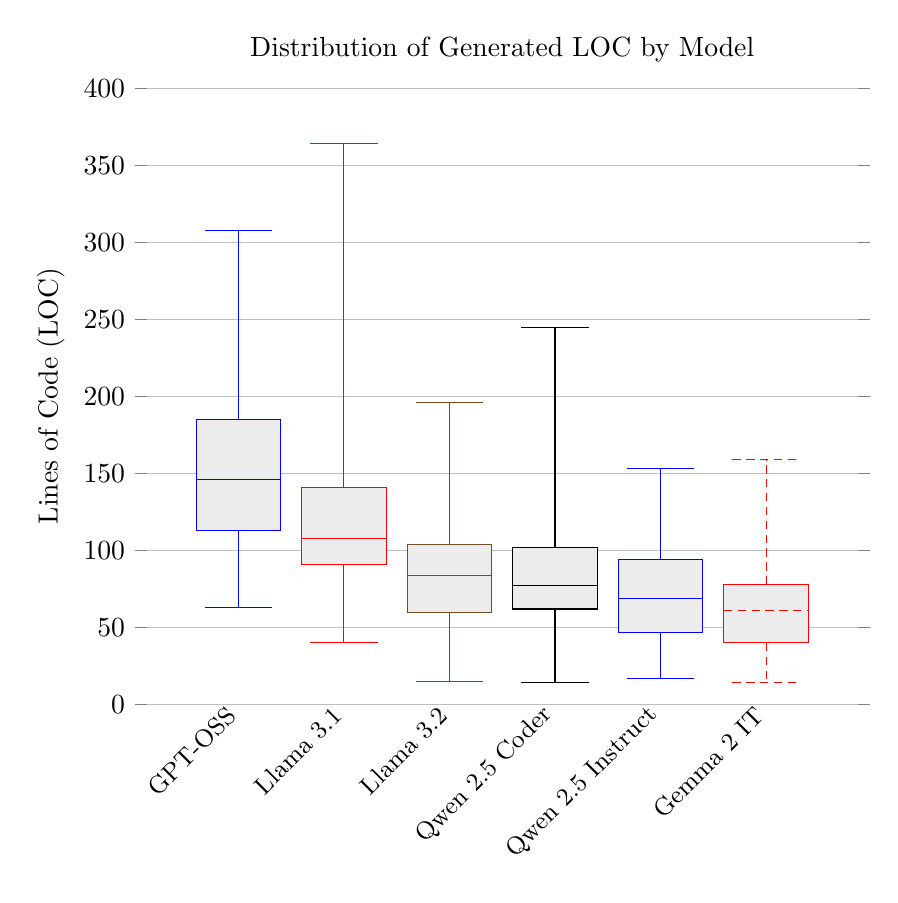
\begin{tikzpicture}
    \begin{axis}[
        title={Distribution of Generated LOC by Model},
        width=0.9\columnwidth, 
        boxplot/draw direction=y,
        x axis line style={opacity=0},
        xtick style={draw=none},
        xticklabel style={rotate=45, anchor=east, font=\small},
        ylabel={Lines of Code (LOC)},
        xtick={
            1,2,3,4,5,6
        },
        xticklabels={
            GPT-OSS,
            Llama 3.1,
            Llama 3.2,
            Qwen 2.5 Coder,
            Qwen 2.5 Instruct,
            Gemma 2 IT
        },
        ymin=0,
        ymajorgrids=true,
        boxplot/every box/.style={solid, fill=gray!15},
    ]
    
    % GPT-OSS 120B
    \addplot+[
      boxplot prepared={
        lower whisker=63,
        lower quartile=113,
        median=146,
        upper quartile=185,
        upper whisker=308
      }
    ] coordinates {};

    % Llama 3.1 8B
    \addplot+[
      boxplot prepared={
        lower whisker=40,
        lower quartile=91,
        median=108,
        upper quartile=141,
        upper whisker=364
      }
    ] coordinates {};

    % Llama 3.2 1B
    \addplot+[
      boxplot prepared={
        lower whisker=15,
        lower quartile=60,
        median=84,
        upper quartile=104,
        upper whisker=196
      }
    ] coordinates {};

    % Qwen Coder 32B
    \addplot+[
      boxplot prepared={
        lower whisker=14,
        lower quartile=62,
        median=77,
        upper quartile=102,
        upper whisker=245
      }
    ] coordinates {};

    % Qwen 7B
    \addplot+[
      boxplot prepared={
        lower whisker=17,
        lower quartile=47,
        median=69,
        upper quartile=94,
        upper whisker=153
      }
    ] coordinates {};

    % Gemma 2 2B
    \addplot+[
      boxplot prepared={
        lower whisker=14,
        lower quartile=40,
        median=61,
        upper quartile=78,
        upper whisker=159
      }
    ] coordinates {};

    \end{axis}
  \end{tikzpicture}
  \caption{Box plot of generated Lines of Code (LOC) distribution for each model, showing min, quartiles, median, and max.\\}
  \label{fig:loc-boxplot}
\end{figure}

\newpage
The correlation between model size and code length is evident: \textit{GPT-OSS 120B}, the largest model tested, consistently produces the longest code, while the smallest models (\textit{Gemma 2 2B IT} and \textit{Llama 3.2 1B Instruct}) produce the most compact implementations. Interestingly, when comparing this LOC data with the pattern detection rates from Table III, we observe that \textit{GPT-OSS 120B} leads in both metrics (\textbf{41\%} pattern detection rate and \textbf{152.09} mean LOC), suggesting that longer code may provide more opportunities for pattern implementations or that the model's tendency toward more elaborate solutions manifests in both dimensions.


\subsection{Pattern Category Analysis}
When grouping the detected patterns into their GoF categories, we observe a slight skew towards \textbf{Behavioral} (\textbf{48.9\%}) and \textbf{Creational} (\textbf{42.7\%}) patterns. \textbf{Structural} patterns were significantly less common, accounting for only \textbf{8.4\%} of all detected instances.

Table \ref{tab:category-distribution} shows this breakdown by model. This suggests that LLMs are adept at generating patterns for object creation and communication, while complex structural compositions are rare. The high number for the \textbf{Creational} category is driven almost entirely by the \textbf{Builder} pattern, and the high \textbf{Behavioral} count is driven by \textbf{State} and \textbf{Command}.

% Table: Category Distribution
\begin{table}[htbp]
 \centering
 \caption{Pattern Category Distribution by Model}
 \label{tab:category-distribution}
 \setlength{\tabcolsep}{3pt} % Reduce column spacing
 \small % Use smaller font
 \begin{tabular}{@{}lrrrrrrr@{}}
    \toprule
    & \multicolumn{6}{c}{Model} & \\
    \cmidrule(r){2-7}
    Category &
    \rotatebox{60}{Gemma} &
    \rotatebox{60}{GPT-OSS} &
    \rotatebox{60}{Llama 3.1} &
    \rotatebox{60}{Llama 3.2} &
    \rotatebox{60}{Qwen Inst} &
    \rotatebox{60}{Qwen Coder} &
    \textbf{Total} \\
    \midrule
    Creational & 4 & 20 & 6 & 5 & 11 & 10 & \textbf{56} \\
    Structural & 1 & 2 & 2 & 2 & 2 & 2 & \textbf{11} \\
    Behavioral & 7 & 29 & 6 & 5 & 8 & 9 & \textbf{64} \\
    \midrule
    \textbf{Total} & \textbf{12} & \textbf{51} & \textbf{14} & \textbf{12} & \textbf{21} & \textbf{21} & \textbf{131} \\
    \bottomrule
 \end{tabular}
\end{table}


%%%%%%%%%%%%%%%%%%%%%%%%%%%%%%%%%%%%%%%%%%%%%%%%%%%%%%%%%%%%%%%%%%%%%%%%%%%%%%%%
% --- V. DISCUSSÃO ---
% Esta secção foi ATUALIZADA com os novos dados
%%%%%%%%%%%%%%%%%%%%%%%%%%%%%%%%%%%%%%%%%%%%%%%%%%%%%%%%%%%%%%%%%%%%%%%%%%%%%%%%
\section{Discussion}
The results of our analysis provide several insights into the current state of LLM-generated code. We interpret these findings and their implications for software engineering.

First, the low overall pattern detection rate (\textbf{18.2\%}) strongly implies that LLMs favor simpler, more direct implementations over architecturally complex solutions. In \textbf{81.8\%} of cases, the models generated code with no identifiable GoF patterns, opting for straightforward procedural or class-based logic. This may be desirable for simple tasks but raises concerns about scalability and maintainability for more complex, system-level prompts.

Second, a clear pattern bias exists. The heavy favoritism shown towards the \textbf{Builder} (\textbf{44} occurrences), \textbf{State} (\textbf{29}), and \textbf{Command} (\textbf{24}) patterns, coupled with the complete absence of \textbf{13} other GoF patterns (such as Observer, Composite, or Decorator), suggests that the models' training data or internal reasoning is skewed. The Builder pattern, for instance, may be common due to its frequent use in data classes and APIs (e.g., \textit{StringBuilder}), making it a high-frequency token sequence in training corpora.

Third, model architecture and training matter. The \textbf{30-point} variance in detection rates between \textit{GPT-OSS 120B} (\textbf{41\%}) and \textit{3.2 1B Instruct} / \textit{Gemma 2 2B IT} (\textbf{11\%}) demonstrates that not all models are equal in their ability or tendency to reproduce structured designs. This suggests that the scale of the model, its training data, and its fine-tuning process all have a measurable impact on the design quality of the code it produces.

Finally, the impact of training data is further highlighted by the missing patterns. The \textbf{13} undetected patterns (including common ones like \textbf{Observer}, \textbf{Composite}, and \textbf{Decorator}) are not necessarily more complex, but they may be less common in the open-source codebases used for training.

These findings suggest that while LLMs are capable of generating functional code, they cannot yet be relied upon to make sophisticated, high-level design decisions autonomously. The code they produce reflects the most common patterns found in public data, not necessarily the most appropriate design for a given problem.


% --- VI. CONCLUSÃO E TRABALHO FUTURO ---
\section{Conclusion and Future Work}
\subsection{Conclusion}
This study presented a pioneering empirical analysis of the spontaneous emergence of the 23 "Gang of Four" (GoF) design patterns in Java code generated by six large language models (LLMs). Through a systematic methodology involving 100 neutral prompts and the rigorous validation of the \textit{Design Pattern Finder} (DPF) static analysis tool, we obtained quantitative insights into the design tendencies of current LLMs.

The primary conclusions are clear and significant. The most prominent finding is that LLMs, when not explicitly instructed, tend to avoid architectural complexity. The vast majority of the generated code, \textbf{81.8\%}, contained no identifiable GoF patterns, favoring straightforward procedural implementations. This raises questions about the scalability and maintainability of LLM-generated code for more complex problems.

Furthermore, the diversity of patterns was extremely low. Only \textbf{10} of the 23 GoF patterns were detected across all 600 files. The distribution was heavily concentrated, with the \textbf{Builder}, \textbf{State}, and \textbf{Command} patterns alone accounting for nearly \textbf{78\%} of all detected instances. Surprisingly, \textbf{13} GoF patterns—including fundamental ones like \textbf{Observer}, \textbf{Composite}, and \textbf{Decorator}—were not detected at all.

The choice of LLM also has a measurable impact on design. The \textit{GPT-OSS 120B} model, the largest one tested, exhibited the highest pattern detection rate at \textbf{41\%} and also produced the longest code, with a mean of \textbf{152.09 LOC}. In contrast, smaller models like \textit{Llama 3.2 1B} and \textit{Gemma 2 2B IT} had the lowest rates at \textbf{11\%}. These results suggest that current LLMs are not yet reliable for making sophisticated, autonomous software design decisions. Their behavior appears to reflect the statistically most common patterns found in their training data, rather than a deep understanding of design problems and the application of the most appropriate solution.

\subsection{Future Work}
The results of this study open several promising paths for future research, which are essential for understanding and improving the architectural quality of AI-generated code. This study focused on neutral prompts; a logical next step is to investigate the ability of LLMs to correctly implement design patterns, especially the \textbf{13} that were absent, when explicitly instructed to do so. Our analysis was quantitative, focusing on detection. Future research should pivot to a qualitative analysis to assess whether the detected patterns were, in fact, the most appropriate design solution for the problem proposed by the prompt.

This analysis was also limited to Java. It would be valuable to replicate this study in other object-oriented languages, such as Python or C\#, to determine if the observed pattern bias is universal or specific to the Java ecosystem. The prompts used described relatively contained programming problems. Future studies should use prompts that describe more complex, larger-scale systems to investigate whether inherently more complex problems force LLMs to utilize the structural patterns that were missing in this study. Finally, a specific investigation into why common patterns like \textit{Observer} and \textit{Decorator} were not generated is warranted. This could involve analyzing the training corpora or fine-tuning models to verify if they can learn and apply these crucial design concepts.


%%%%%%%%%%%%%%%%%%%%%%%%%%%%%%%%%%%%%%%%%%%%%%%%%%%%%%%%%%%%%%%%%%%%%%%%%%%%%%%%
% --- REFERÊNCIAS ---
%%%%%%%%%%%%%%%%%%%%%%%%%%%%%%%%%%%%%%%%%%%%%%%%%%%%%%%%%%%%%%%%%%%%%%%%%%%%%%%%
\newpage
\bibliographystyle{IEEEtran}
\bibliography{myreferences}

\balance

\end{document}